% -*- mode: fundamental -*-

% Slides accompanying "Learn RISC-V CPU Implementation and BSV" book
% Copyright (c) 2024 Rishiyur S. Nikhil, All Rights Reserved

% -*- mode: fundamental -*-

% Slides accompanying "Learn RISC-V CPU Implementation and BSV" book
% Copyright (c) 2024 Rishiyur S. Nikhil, All Rights Reserved

% This is a preamble shared by all the slide decks

\documentclass[10pt, aspectratio=169]{beamer}

% \documentclass[17pt]{beamer}

% Avail. font sizes: 8pt, 9pt, 10pt, 11pt, 12pt, 14pt, 17pt, 20pt.
% Default font size is 11pt (= 22pt in full screen mode).

\usepackage{verbatim}
\usepackage{fancyvrb}
\usepackage{listings}

% ================================================================
% Themes

\usetheme{Madrid}          % Line at bottom: Author (affiliation), OptTitle, Conf, page 

% \usetheme{Copenhagen}    % Same as Madrid except bottom line: Author, OptTitle

% \usetheme{Berkeley}    % Takes up 1-inch border on left and top

% ----------------
% colorthemes
% (default), beaver, beetle, seahorse, wolverine

\usecolortheme{seahorse}

% ================================================================
% Customization: show table of contents before each section
% Use \AtBeginSubsection    to show before each subsection

% \AtBeginSection[]
% {
%   \begin{frame}
%     \frametitle{Table of Contents}
%     \tableofcontents[currentsection]
%   \end{frame}
% }

% ================================================================

% ----------------
% The bsc compiler and BSV language
\newcommand{\bsc}{\emph{bsc}}
\newcommand{\BSV}{\bf{BSV}}
% ----------------
% ITALICISE WORDS
\newcommand{\ie}{\emph{i.e.,}}
\newcommand{\eg}{\emph{e.g.,}}
\newcommand{\Eg}{\emph{E.g.,}}
\newcommand{\etc}{\emph{etc.}}
\newcommand{\via}{\emph{via}}
\newcommand{\vs}{\emph{vs.}}

% ----------------
% EMPTY BOXES OF VARIOUS WIDTHS, FOR INDENTATION

\newcommand{\hm}{\hspace*{1em}}
\newcommand{\hmm}{\hspace*{2em}}
\newcommand{\hmmm}{\hspace*{3em}}
\newcommand{\hmmmm}{\hspace*{4em}}

% ----------------
% Convenient widths

\newlength{\hlessmm}
\setlength{\hlessmm}{\textwidth}
\addtolength{\hlessmm}{-2em}

\newlength{\hlessmmm}
\setlength{\hlessmmm}{\textwidth}
\addtolength{\hlessmmm}{-3em}

\newlength{\hlessmmmm}
\setlength{\hlessmmmm}{\textwidth}
\addtolength{\hlessmmmm}{-4em}

% ================================================================
% Title page

\title[Learn CPU design \& BSV]{Learn RISC-V CPU Implementation and BSV}

\subtitle{(BSV: a High-Level Hardware Design Language)}

\author[{\copyright} R.S.Nikhil]{Rishiyur S.~Nikhil}
% \institute{Bluespec, Inc.}

% Date is set differently in each slide deck

% \logo{
\includegraphics[height=0.6cm]{../Figures/Bluespec_Logo_2022-10}}

% End of preamble
% ****************************************************************


\date{L8: RISC-V: GPRs and CSRs}

% ****************************************************************

\begin{document}

% ================================================================

\begin{frame}
 \titlepage

 \begin{center}
  
\includegraphics[height=1cm]{Bluespec_Logo_2022-10}
 \end{center}

\end{frame}

% ================================================================

% -*- mode: fundamental -*-

% ================================================================

\begin{frame}[fragile]
\frametitle{Reminders}

\footnotesize

Please git clone: \url{https://github.com/rsnikhil/Learn_Bluespec_and_RISCV_Design} \\
(git pull for latest version).  Repsitory structure:

\vspace{1ex}

\begin{minipage}{0.5\textwidth}\scriptsize
\begin{Verbatim}[frame=single, numbers=left]
    ./Book_BLang_RISCV.pdf
      Slides/
          Slides_01_Intro.pdf
          Slides_02_ISA.pdf
          ...
      Exercises/
          Ex-03-A-Hello-World/
          Ex-03-B-Top-and-DUT/
          ...
      Code/
          src_Top/
          src_Drum/
          src_Fife/
          src_Common/
          ...
      Doc/Installing_bsc_Verilator_etc.{adoc,html}
\end{Verbatim}
\end{minipage}
\hm
\begin{minipage}{0.45\textwidth}
\begin{itemize}

 \item Slides and Exercise are numbered in sync with book Chapter numbers.

 \item For Exercises, please see Appendix E of the book.  Some (not
       all) exercises have associated code in the {\tt Exercises/}
       directory.

\end{itemize}
\end{minipage}

\vspace{2ex}

To compile and run the code for exercises, Drum and Fife, please make sure you have installed:

\begin{itemize}

 \item \emph{bsc} compiler (see \url{https://github.com/B-Lang-org/bsc})

 \item Verilator compiler (see \url{https://www.verilator.org/})
\end{itemize}

\footnotesize

\end{frame}

% ================================================================

\begin{frame}
\frametitle{Chapter Roadmap}

\footnotesize

\begin{center}
\frame{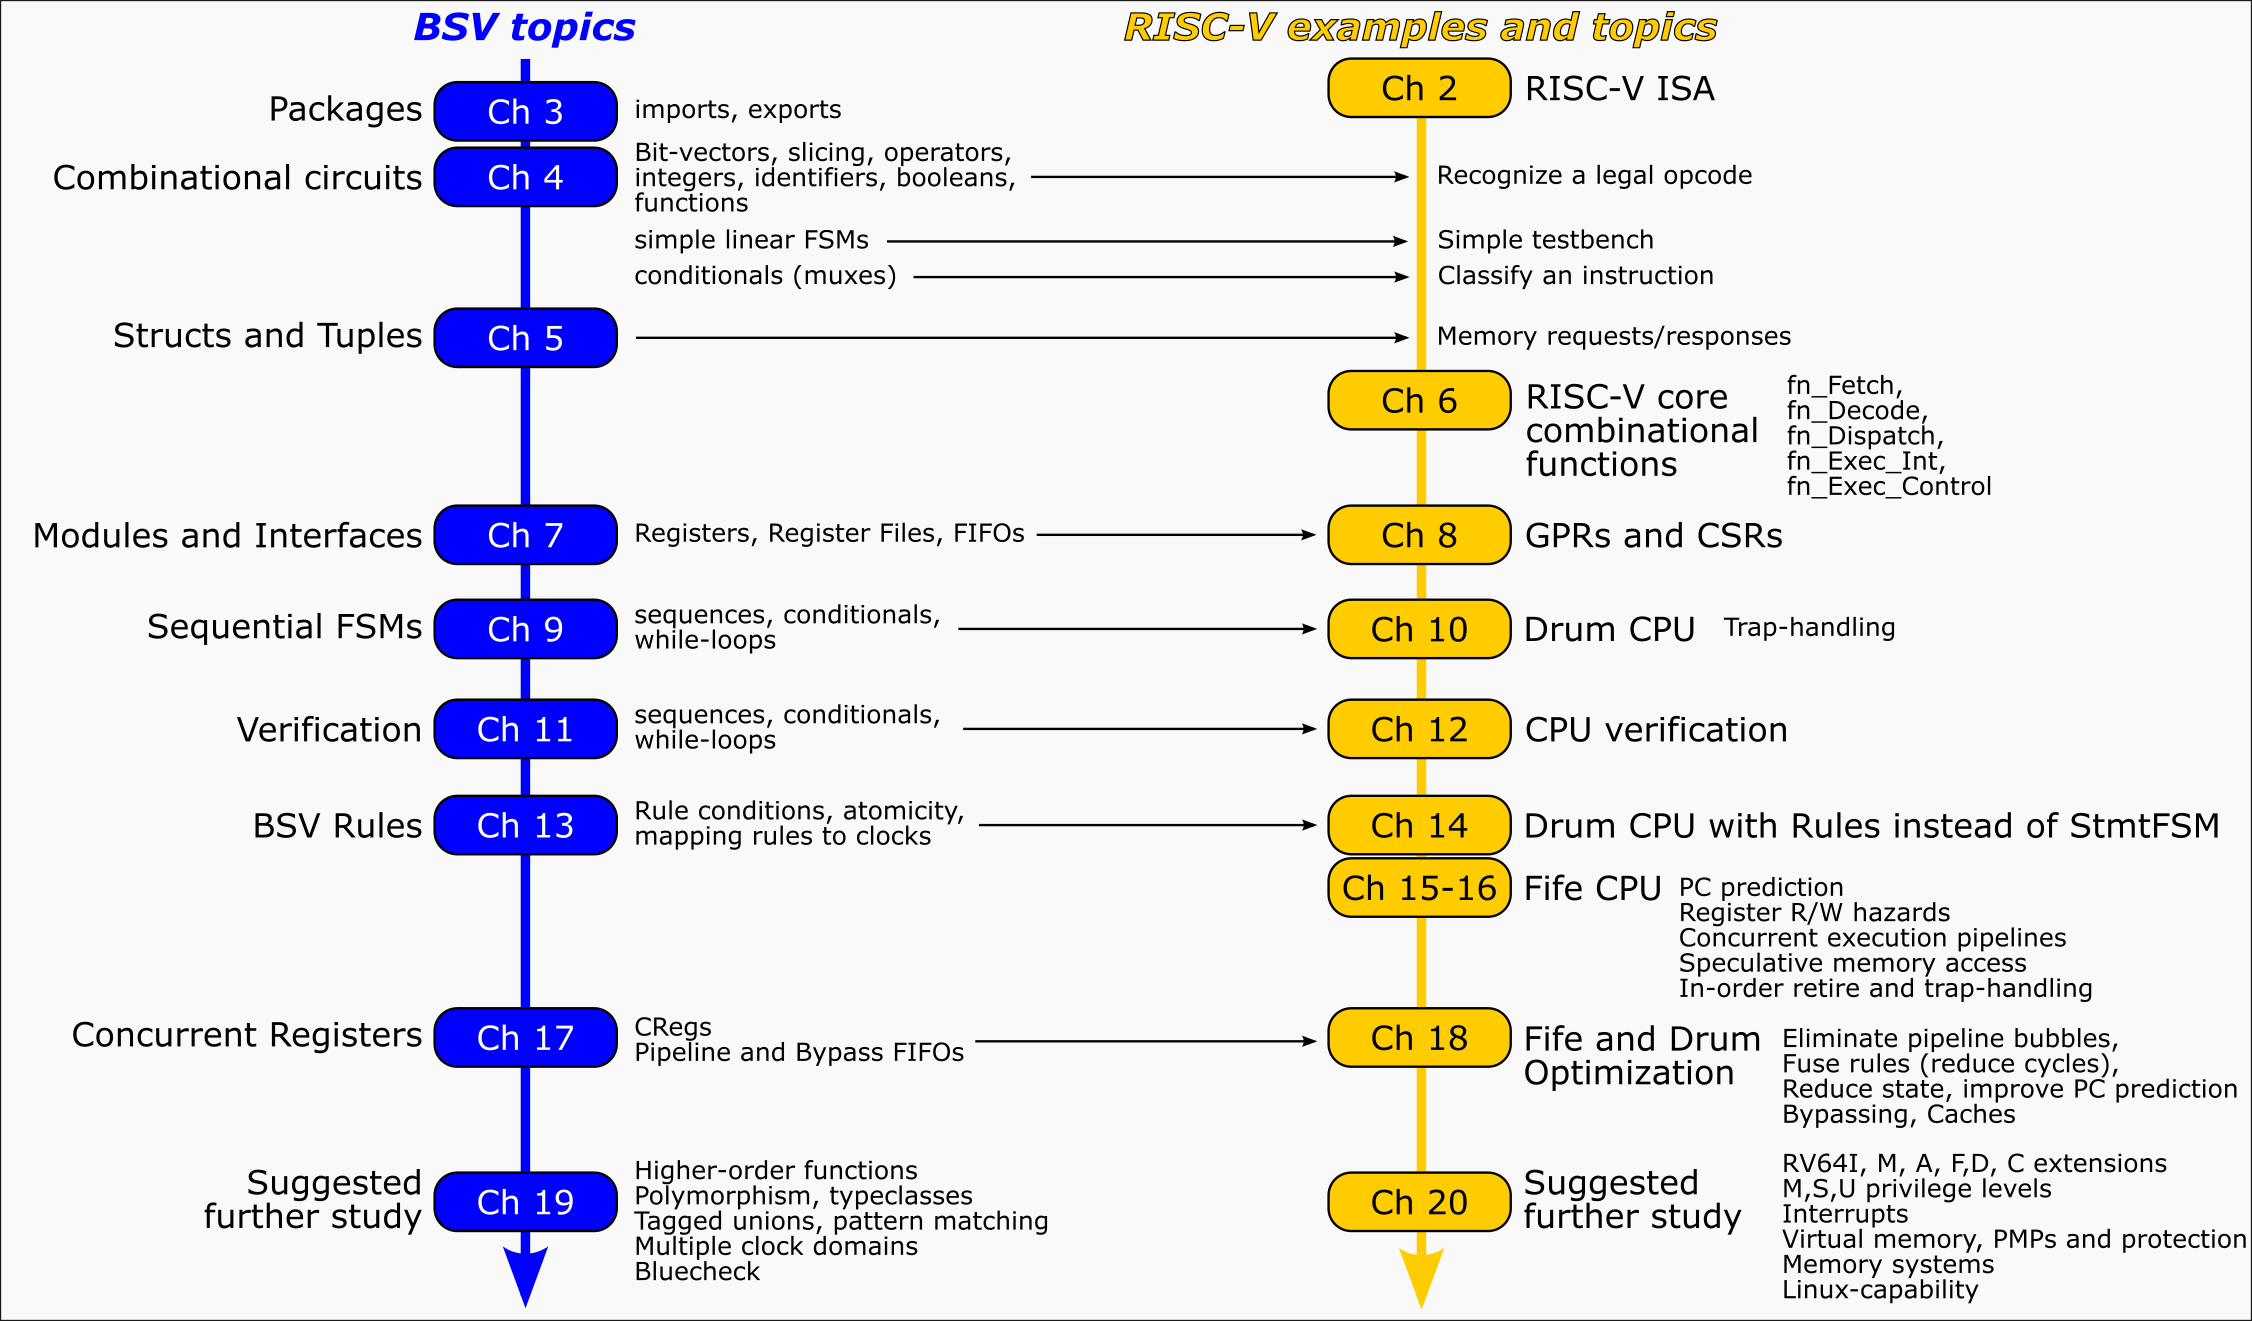
\includegraphics[height=0.825\textheight]{Fig_Chapter_Roadmap}}
\end{center}

\end{frame}

% ================================================================


% ================================================================

\begin{frame}
\frametitle{Flow of information between stages in Drum and Fife}

\footnotesize

\begin{center}
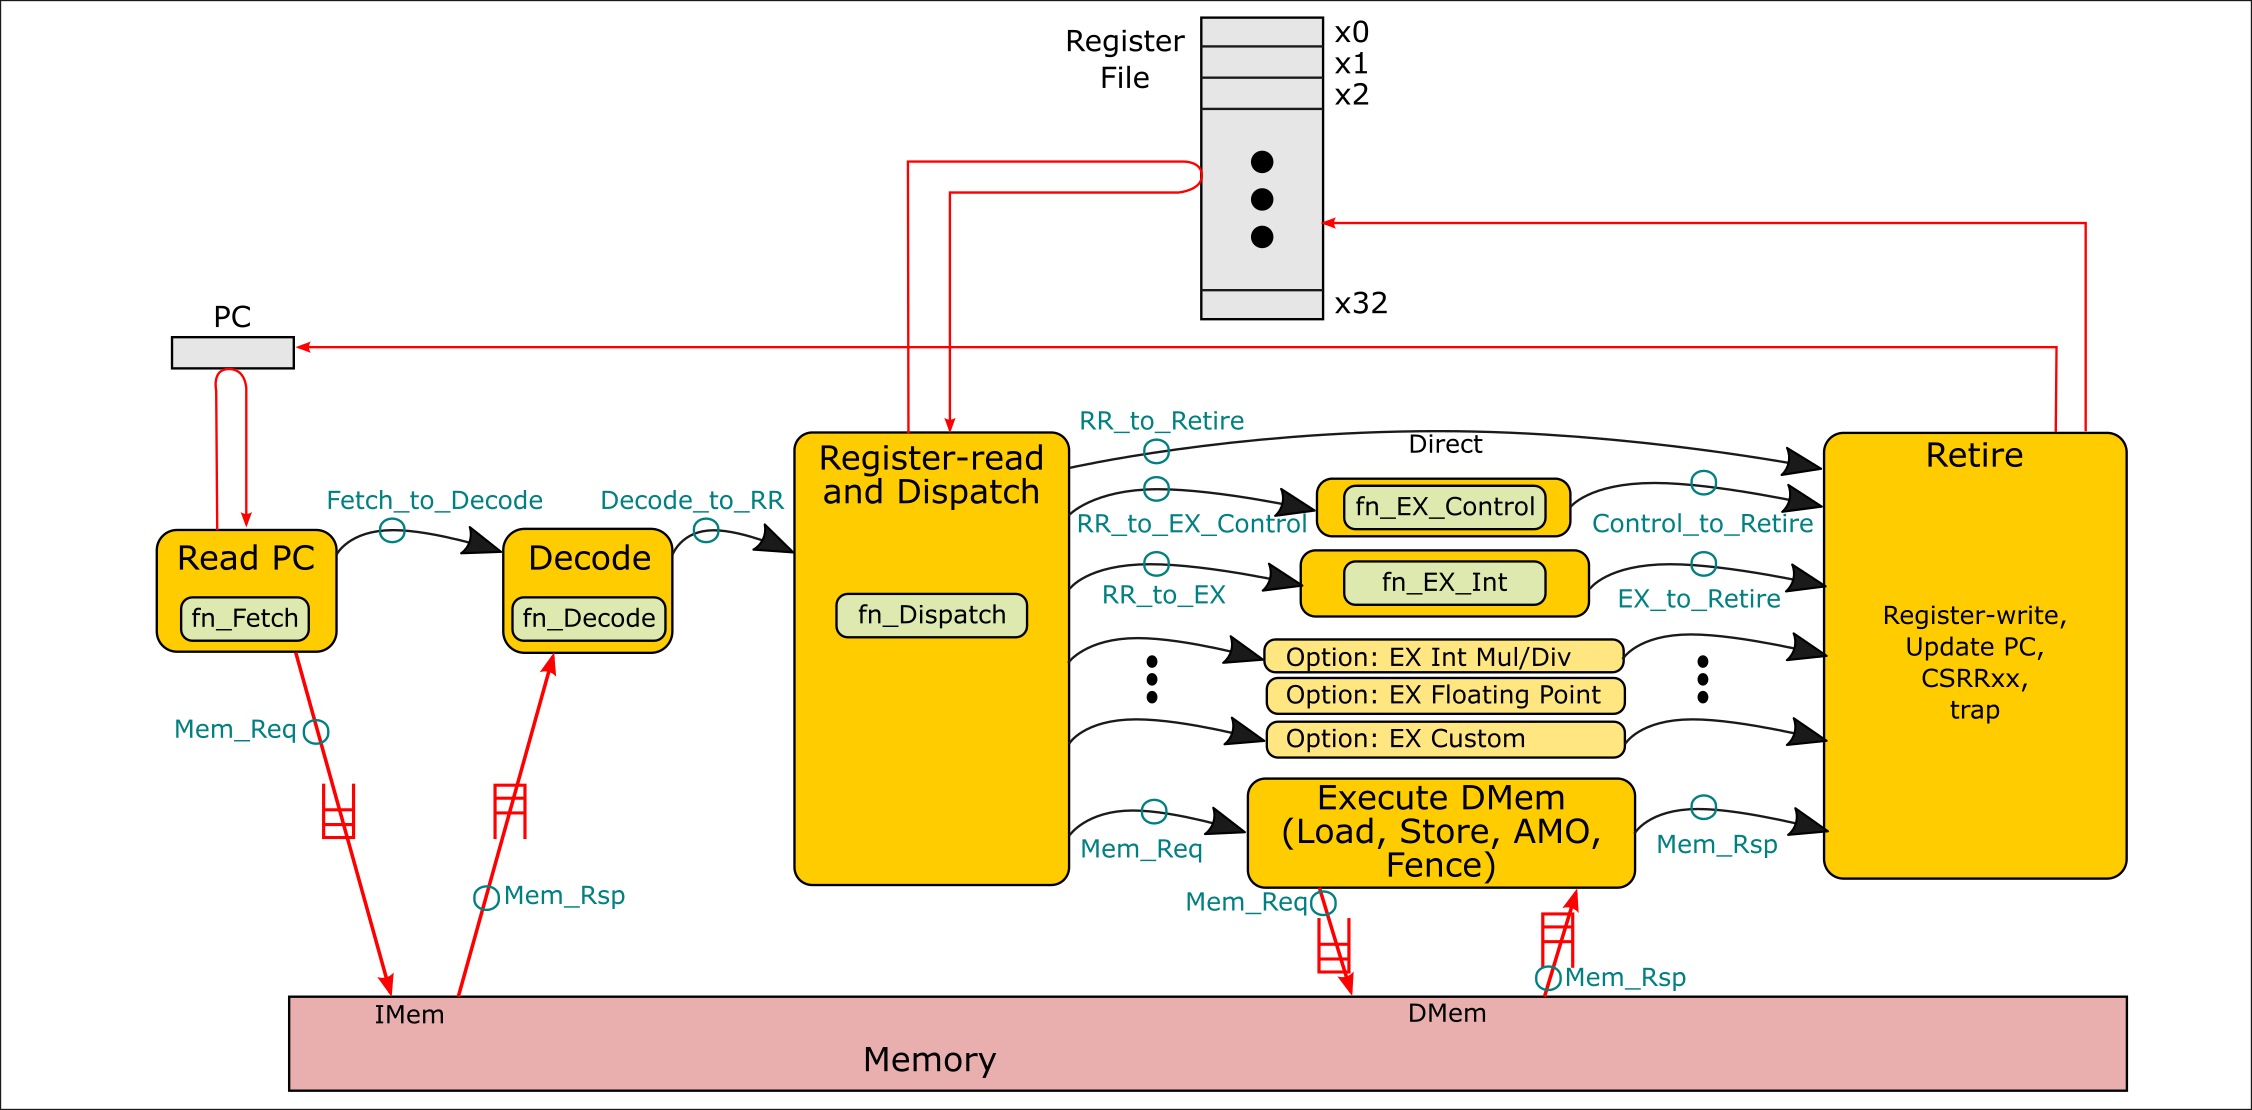
\includegraphics[height=0.6\textheight]{Fig_Instr_Exec_w_structs}
\end{center}

\end{frame}

% ================================================================

\begin{frame}
\frametitle{Table of Contents}

\tableofcontents

\end{frame}

% ****************************************************************

\section{GPRs (General Purpose Registers)}

% ================================================================

\begin{frame}

\begin{center}
  {\LARGE GPRs (General Purpose Register file)}
\end{center}

\end{frame}

% ================================================================

\begin{frame}[fragile]
\frametitle{RISC-V: Interface for the {\tt mkGPRs} module}

\footnotesize

Although we could have just used the {\BSV} library ``{\tt RegFile}''
interface, we define a new interface that specializes it to the
particular types in our application, and with more meaningful names:

\vspace{2ex}

\SHOWCODE{../Code_Extracts/GPRs_IFC.tex}

\vspace{2ex}
Note:
\begin{itemize}

 \item This is a polymorphic module; ``{\tt xlen}'' can be
   instantiated with the numeric type 32 for RV32 and 64 for RV64.

 \item Each method in a module interface can be invoked at most once
   in a clock.  We will need to read {\tt rs1} and {\tt rs2} registers
   simultaneously, and so we provide a separate method for each.

\end{itemize}

\end{frame}

% ================================================================

\begin{frame}[fragile]
\frametitle{RISCV: Register x0 is a special case}

\footnotesize

In RISC-V ISA semantics, register x0 (index 0) is defined as ``always
zero''. Any value written to x0 is ignored/discarded, and any read
from x0 always returns 0.

\vspace{1ex}

The {\tt mkGPRs} module is a thin wrapper for the {\BSV} library {\tt
  mkRegFileFull} module, treating index 0 as a special case.

\vspace{1ex}

\SHOWCODE{../Code_Extracts/mkGPRs.tex}

\end{frame}

% ================================================================

\begin{frame}
\frametitle{\EmojiExercise \hmm Exercise break}

Please see Appendix E, Exercise Ex-08-A-GPR-Register-Files.

\end{frame}

% ****************************************************************

\section{CSRs (Control and Status Registers)}

% ================================================================

\begin{frame}[fragile]
\frametitle{RISC-V: CSR addresses}

\footnotesize

A CSR address is 12-bits wide (taken from {\tt instr[31:20]} in CSRRxx instructions).

\vspace{2ex}

Here are the addresses for the CSRs we need for exception-handling:

\vspace{2ex}

\SHOWCODE{../Code_Extracts/csr_addrs.tex}

\end{frame}

% ================================================================

\begin{frame}[fragile]
\frametitle{RISC-V: Interface to the {\tt mkCSRs}}

\footnotesize

The interface methods for {\tt mkCSRs} reflects the way we use CSRs:

\vspace{1ex}

\SHOWCODESCRIPT{../Code_Extracts/CSRs_IFC.tex}

\end{frame}

% ================================================================

\begin{frame}[fragile]
\frametitle{RISC-V: CSRs: General considerations}

\footnotesize

\vspace{2ex}

Technically, there can be $2^{12}$ (= 4096) CSRs.

\vspace{1ex}

In Drum/Fife, we implement hardly a dozen CSRs.

\vspace{1ex}

Even high-end CPUs may implement around hundred CSRs.

\vspace{1ex}

Further,
\begin{itemize}

\item The addresses of CSRs that we do implement are not consecutive.

\item What happens when we read/write a CSR may vary widely for
  different CSRs and may have CSR-specific side effects.  (See
  Sections 2.3, 2.4 and 2.6 in of the Privileged ISA Specification.)

\end{itemize}

\vspace{2ex}

Thus, we cannot use, say, the library {\tt RegFile} module.

\vspace{1ex}

Instead, we implement CSRs using an \emph{ad hoc} collection of
separate registers, and \emph{ad hoc} read/write logic for each CSR.
Here is the code for the CSRs we need for exception-handling:

\vspace{2ex}

\SHOWCODE{../Code_Extracts/Reg_csr_xxx}

\end{frame}

% ================================================================

\begin{frame}
\frametitle{RISC-V: {\tt mkCSRs} module}

\footnotesize

\begin{center}\large
 Please view the actual code in: \hm {\tt Code/src\_Common/CSRs.bsv}
\end{center}

\vspace{2ex}

Start by viewing the internal functions \\
\hmm {\tt fn\_fav\_csr\_read()} \\
and \\
\hmm {\tt fn\_fav\_csr\_write()} \\
which constitute the basic read/write actions.

\vspace{2ex}

Then see how these functions are used by the interface methods.

\end{frame}

% ================================================================

\begin{frame}
\frametitle{\EmojiExercise \hmm Exercise break}

Please see Appendix E, Exercise Ex-08-B-CSRs.

\end{frame}

% ****************************************************************

% -*- mode: fundamental -*-

% Slides accompanying "Learn RISC-V CPU Implementation and BSV" book
% Copyright (c) 2024 Rishiyur S. Nikhil, All Rights Reserved

% This is a postamble shared by all the slide decks

% ================================================================

\begin{frame}

\begin{center}
  {\LARGE End}
\end{center}

\end{frame}

% ================================================================


% ****************************************************************

\end{document}
% ****************************************************************
